\documentclass{article}
\usepackage[utf8]{inputenc}
\usepackage[icelandic]{babel}
\usepackage[T1]{fontenc}
\usepackage{graphicx}
\usepackage{mathtools}
\usepackage{amsmath}
\usepackage{amssymb}
\usepackage{minted}


\graphicspath{ {./imgs} }
\title{Snake 4 - Viðmótsforritun}
\author{ttb3@hi.is}
\date{\today}


\begin{document}
\maketitle


\section*{Gagnvirkniskröfur notenda}
\subsection*{1.}
\subsubsection*{Gagnvirkni}
    Notandi getur spilað Snake þar sem snákurinn getur borðað mat,stækkað og liðast, 
    snákurinn deyr svo ef hann snertir eitursnák eða klessir á sinn eiginn líkama.
\subsubsection*{Lýsing á verkefni} 
    Í fyrri útgáfu af Snake var aðeins hægt að lengjast en ekki liðast. 
    Með viðbættri liðunarhegðun þarf að breyta stjórnun á snáknum, 
    athuga þarf í hvaða átt snákurinn stefnir og koma í veg fyrir að hann snúi við.

\subsection*{2.}
\subsubsection*{Gagnvirkni}
Notandi getur skráð stigin sín niður ásamt þremur einkennisstöfum,
eins og í gömlum spilakössum.\footnote{Sjá mynd 2.1} Þessi stig eiga að geymast á milli leikja.

\subsubsection*{Lýsing á verkefni}
Hingað til hefur stigafjöldi verið vistaður sjálfkrafa og með enga vísun í notenda.
stigin voru aðeins til staðar frá því að leikurinn hafðist og þangað til að honum var lokað,
ekkert var geymt á milli keyrslna.

\subsection*{3.}
\subsubsection*{Gagnvirkni}
Notandi getur hefnt sín á eitursnákum, öðru hvoru er maturinn sem birtist 'sérstakur'
á þann hátt að þegar notandi borðar sérstaka matinn, 
getur hann ekki dáið og ef snákurinn rekst á eitursnák deyr eitursnákurinn.
Mjög svipuð pæling og stóru doppurnar í pac-man og stjörnur í super mario.
\footnote{Sjá myndir 3.1 og 3.2}

\subsubsection*{Lýsing á verkefni}
Eins og er í leiknum eru eitursnákarnir bara til staðar til að angra og hægja á leiknum.
Eftir nokkrar mínútur af leik voru komnir svo margir eitursnákar að varla var hægt að spila lengur.
Með þessari viðbót ætti að vera hægt að spila lengur, passa þarf bara að gefa ekki of mikið af sérstökum mat.

\subsection*{4.}
\subsubsection*{Gagnvirkni}
Notandi getur pásað leik með mús, space eða escape. 
Þegar notandi pásar leikinn fær viðkomandi yfirlit yfir hversu langur tími er liðinn,
hversu mikinn mat er búið borða, hvar hann er í röðinni með stig á þessum tímapunkti, 
hversu margir eitursnákar hafa birst, hversu margir eitursnákar hafa dáið og hversu mikið af sérstökum mat er búið að borða.

\subsubsection*{Lýsing á verkefni}
Í augnablikinu er bara hægt að pása með músarsmelli, því þarf að breyta í esc og space. 
Þegar notandi pásar núna gerist ekkert nema að leikurinn frýs. Bætist við öll gögnin um leikinn sem eru talin upp í gegnvirknispartinum.

\subsection*{5.}
\subsubsection*{Gagnvirkni}
Startskjár, 
bæta við almennilegum startskjá þar sem hægt er að fá yfirlit yfir stig 
og hugsanlega einhver auka skemmtileg gögn.

\subsubsection*{Lýsing á verkefni}
Leikurinn eins og er notast við startskjá sem er illa gerður, 
eina sem hægt er að sjá er smá texti og eina sem hægt er að gera er að byrja leikinn.
Bæta við stigalista og betra útliti.


\section*{Útlits- og hönnunarkröfur}
Leikurinn eins og hann lítur út núna er forljótur.
\subsection*{1.}
\subsubsection*{Útlitskröfur}
Allir leikjahlutir eiga að notast við sprites frekar en einföld form gerð í javafx.
Það þarf ekki að vera sjúklegur munur á þessum spritum, 
eitur og player snákar geta litið eins út nema með mismunandi litum.

\subsubsection*{Lýsing á kröfu}
Núna eru snákarnir bara kassar með útlínur og maturinn rauðir hringir, mjög ljótt.
Með þessari kröfu mun leikurinn byrja að líta út eins og eitthvað sem er ekki sett saman af smábarni.


\section*{Notendur og persónur}
\subsection*{Notandi 1 - Baldur Jónsson - Bókari}
\subsubsection*{Færni}
\begin{center}
    \begin{tabular}{|p{2cm}|p{9cm}|}
        \hline
        Líkamleg&Baldur er miðaldra en hefur haldið sér í góðu formi og hefur 'venjulega' líkamlega getu\\
        \hline
        Skynjun&Baldur hefur góða sjón en notar gleraugu, hann hefur væga litblindu en ekkert alvarlegt\\
        \hline
        Athygli&Baldur hefur aldrei verið mikill leikjamaður vegna stuttrar þolinmæði en getur týnt sér í verkefnum og leikjum ef þau eru skemmtileg\\
        \hline
    \end{tabular}
\end{center}


\subsubsection*{Hagfræði}
\begin{center}  
        \begin{tabular}{|p{2cm}|p{9cm}|}
        \hline
        Hvatning&Baldur hefur verið að leita sér að afþreyingu þar sem hann þarf að hugsa aðeins meir en þegar hann situr tímunum saman fyrir framan sjónvarpið\\
        \hline
        Ávinningur&Skemmtilegri sunnudagskvöld og langir fundir\\
        \hline
        Kostar&Forritið sjálft kostar Baldur ekki neitt en hann hefur áhyggjur af því að hann gæti fests í því ef það er of skemmtilegt\\
        \hline
    \end{tabular}
\end{center}

\subsection*{Notandi 2 - Dóra Kolbrún - Menntaskólanemi}
\subsubsection*{Hagfræði}
\begin{center}  
    \begin{tabular}{|p{2cm}|p{9cm}|}
    \hline
    Hvatning&Baldur hefur verið að leita sér að afþreyingu þar sem hann þarf að hugsa aðeins meir en þegar hann situr tímunum saman fyrir framan sjónvarpið\\
    \hline
    Ávinningur&Skemmtilegri sunnudagskvöld og langir fundir\\
    \hline
    Kostar&Forritið sjálft kostar Baldur ekki neitt en hann hefur áhyggjur af því að hann gæti fests í því ef það er of skemmtilegt\\
    \hline
\end{tabular}
\end{center}

\section*{Saga}
\subsection*{1.}
Stemmningin var gríðarleg á lokakvöldi OFURNÖRD. 
Við í HÍ vorum einu stigi frá því að jafna HR og allt stefndi í að úrslitin yrðu ákveðin með bráðabana.
Síðasta kastið og HÍ hittir, staðan er 6-6, tími fyrir bráðabana. 
"Hey hver kom með skákborðið, við þurfum það fyrir bráðabanan!" kallaði ég.
Það hefði mátt heyra saumnál detta, enginn hafði tekið skákborðið með.
"Við þurfum að redda nýjum bráðabana asap, eitthvað sem enginn er sjúklega góður í og allir standa jöfnum fæti".

\subsection*{2.}
"HVAÐ GERÐIST HÉR", hrópaði ég, 
"EF MAMMA OG PABBI KOMA AÐ HÚSINU SVONA FÆ ÉG ALDREI AÐ VERA EINN HEIMA AFTUR".
Strákarni störðu til baka á mig fullir af skömm. 
"Sorrý Jón, það er bara aldrei neitt að gera hérna,
það er útaf því sem við ákváðum að mála sófann gulan".
"Ég veit það er ekkert að gera hérna, 
en þið vitið að ég á ekki efni á PS5 og mamma og pabbi leyfa mér ekki að taka smálán..."
"Ég vildi að það væri ehv sem við gætum gert sem væri ódýrara og myndi ekki breyta litnum á sófanum"

\section*{Áþreifanleg sviðsetning}
"Ég er með lausnina á þessu vandamáli", heyrði ég hrópað úr þvögunni. 
Þetta var Kjartan og hann hélt á fartölvu í höndunum. +
"Ég var að forrita Snake, sjáið bara stigalistann, það er enginn nema ég góður í leiknum".
Ég las stigin og sá, það var rétt hjá honum, Kjartan var sá eini með fleiri stig en 30. 
"Jæja það er slegið", sagði ég, "úrslitin verða ákveðin með snake". 
Fólkið brjálaðist úr gleði.

\section*{Teiknimyndasaga}
\begin{center}
    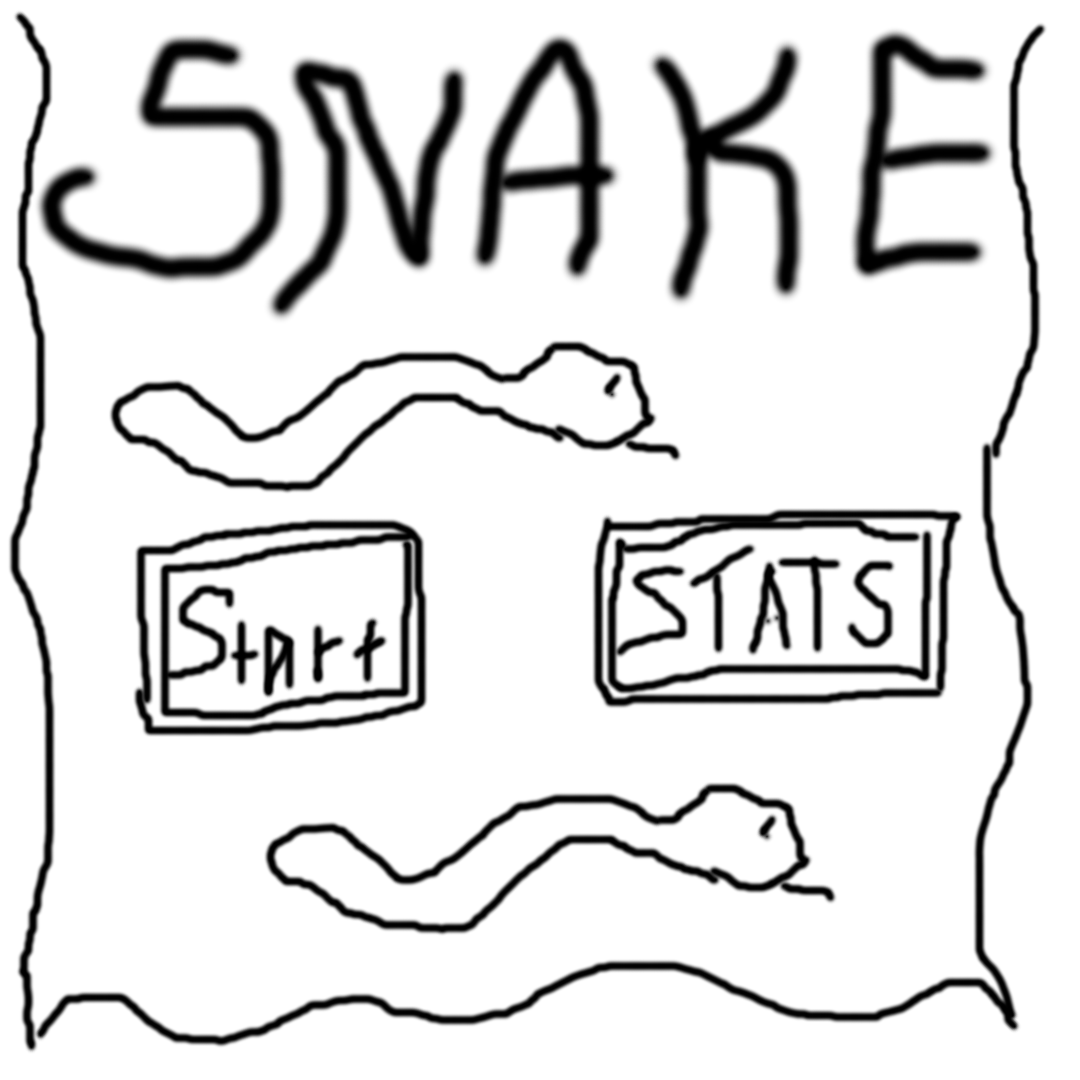
\includegraphics[scale=0.75]{m1.png}\\
    Byrjunarskjár, notandi kíkir á stigin áður en hann byrjar\\
    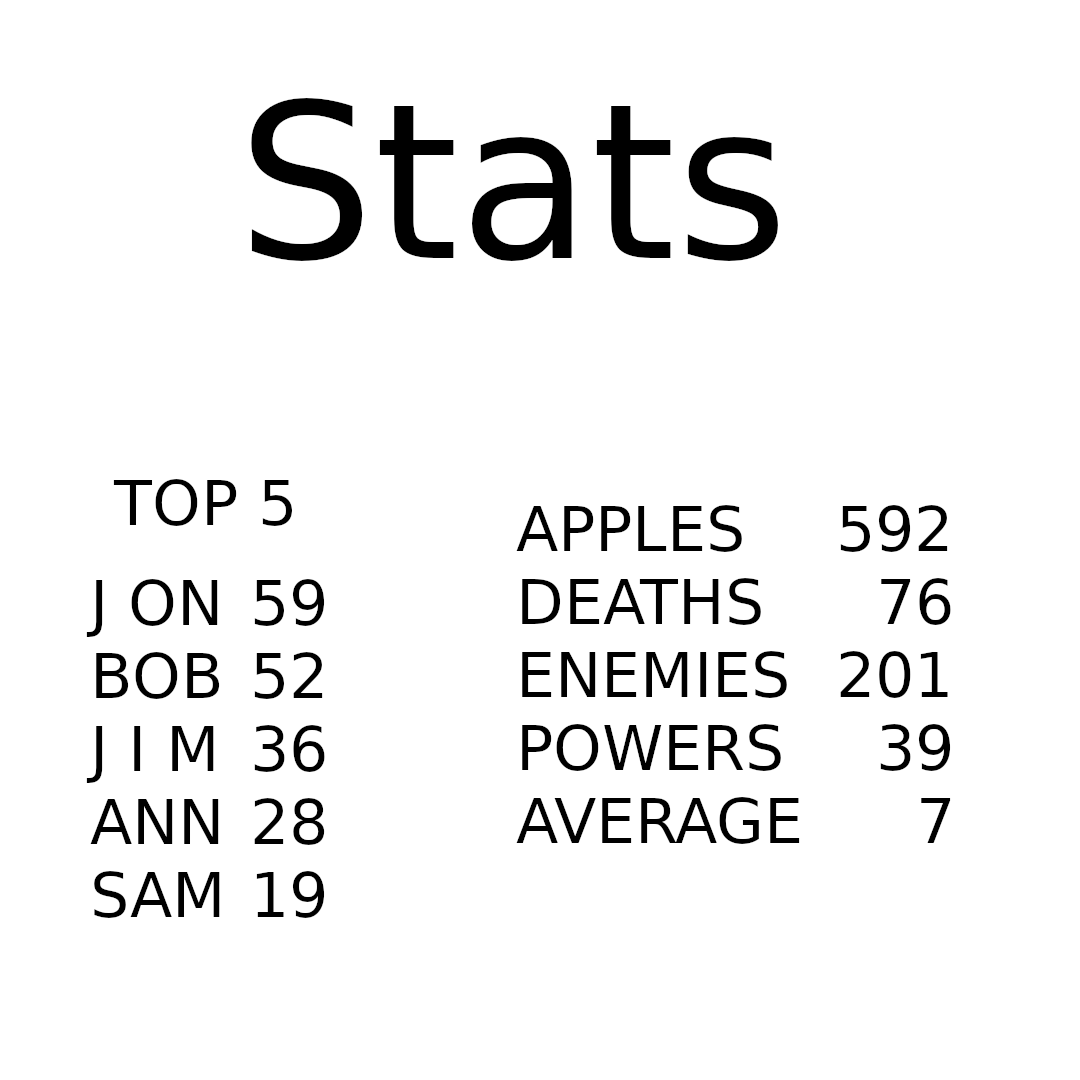
\includegraphics[scale=0.75]{m2.png}\\
    Notandi sér stigafjölda og aðrar upplýsingar, hefur núna markmið fyrir leikinn\\
    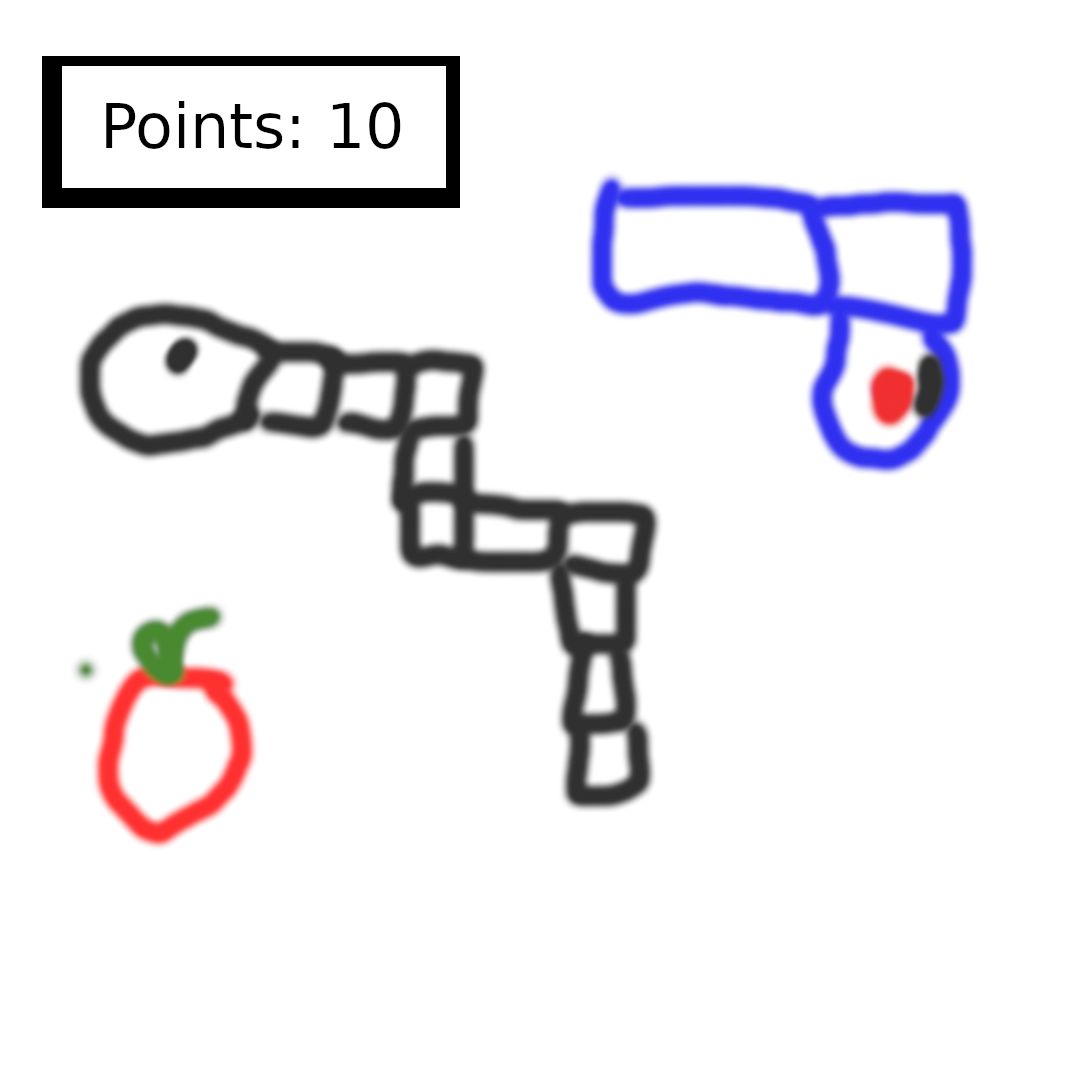
\includegraphics[scale=0.75]{m3.png}\\
    Notandi byrjar leikinn og honum gegnur vel\\
    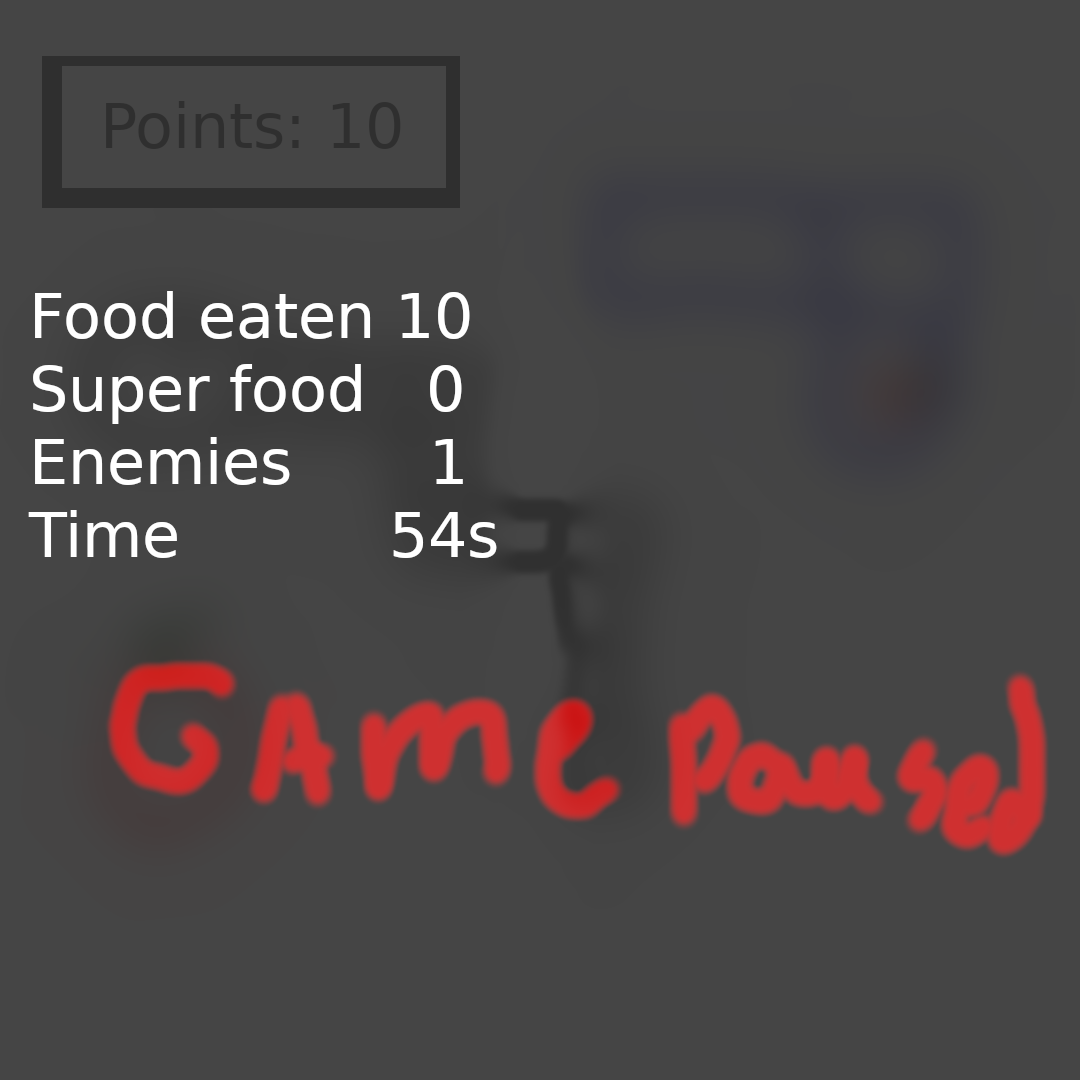
\includegraphics[scale=0.75]{m4.png}\\
    Notandi þarf að hlaupa frá í smá stund, pásar leikinn og sér ýmsa tölfræði\\
    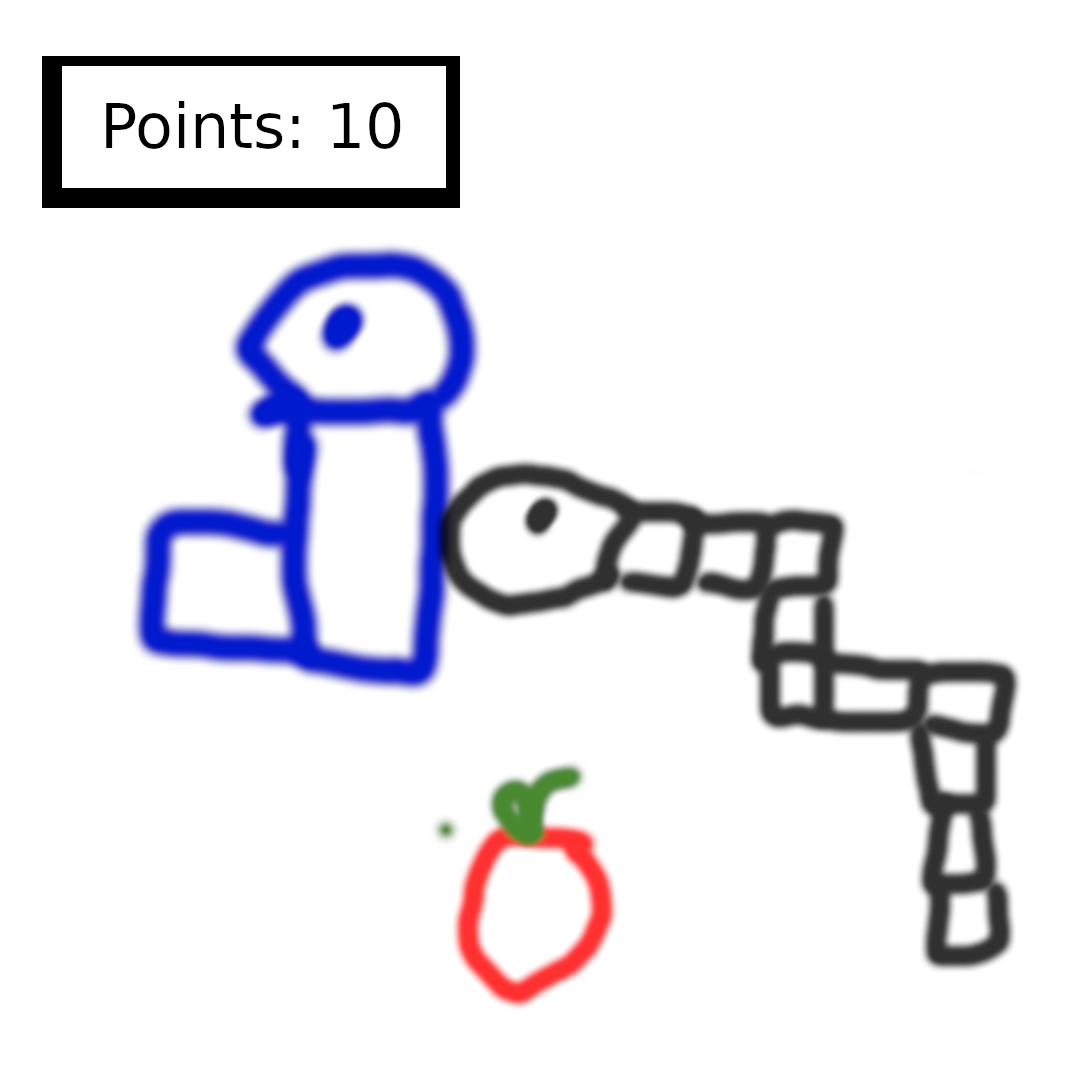
\includegraphics[scale=0.75]{m5.png}\\
    Notandi kemur aftur en er ekki lengur í stuði og klessir á eiginlega strax\\
    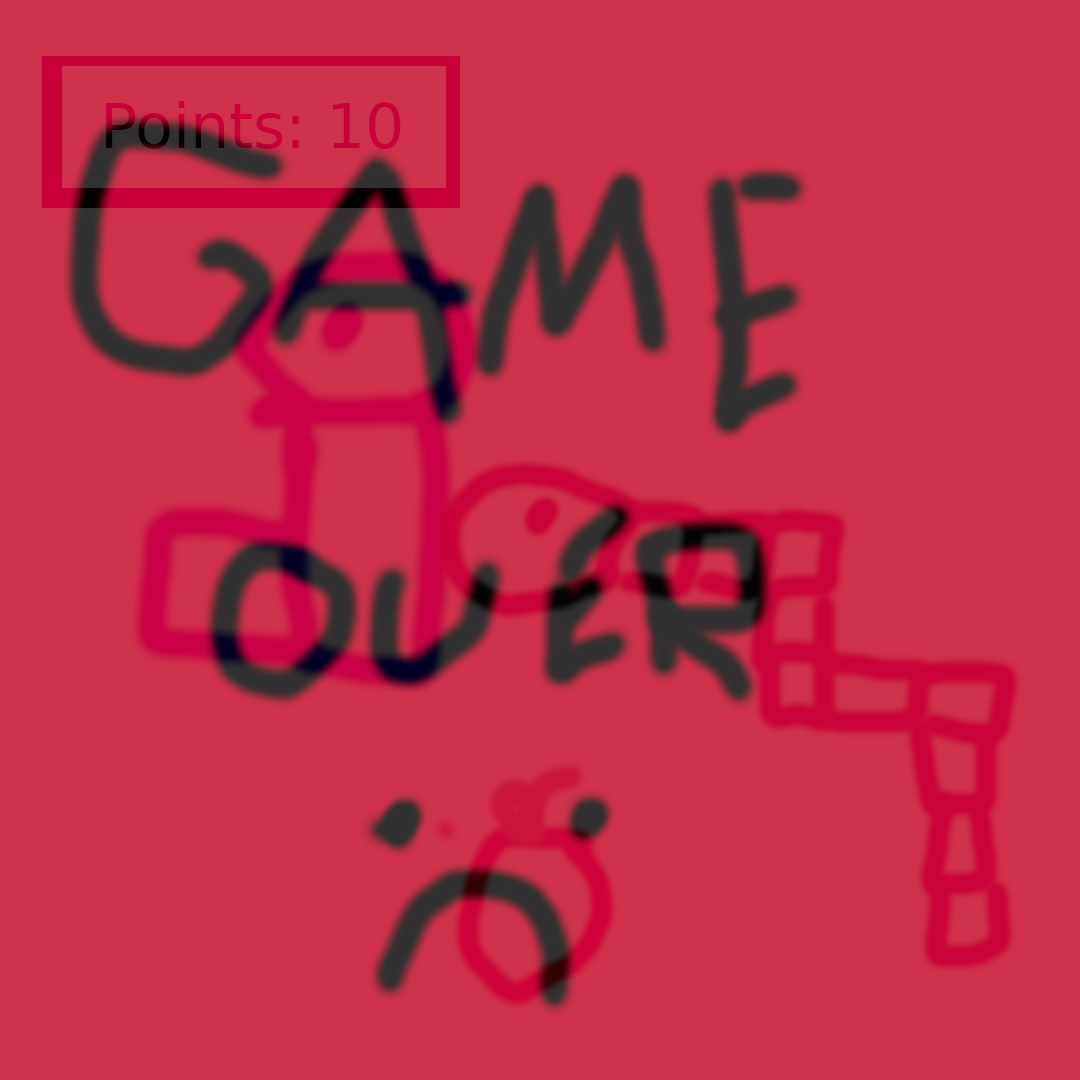
\includegraphics[scale=0.75]{m6.png}\\
    Notandi tapar leiknum\\
\end{center}

\newpage
\section*{Myndir}
\begin{center}
    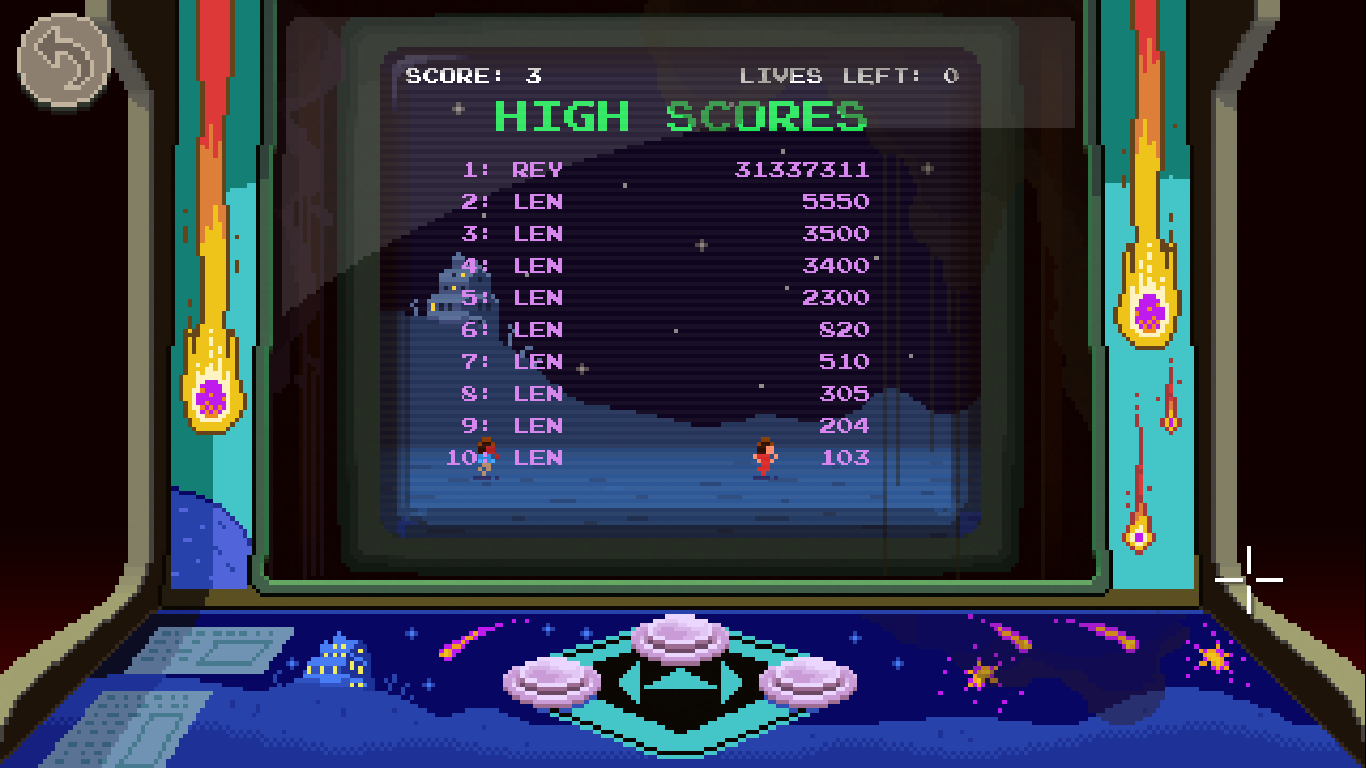
\includegraphics[scale=0.25]{imgs/highscore.png}
\end{center}
mynd 2.1

\begin{center}
    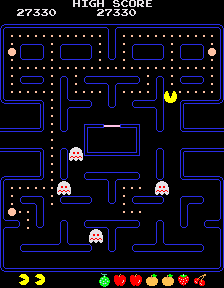
\includegraphics{imgs/pac-man.png}
\end{center}
mynd 3.1
\begin{center}
    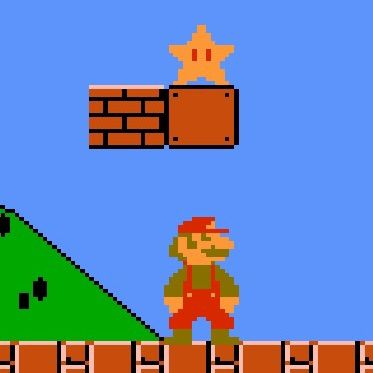
\includegraphics[scale=0.8]{imgs/mario.jpg}
\end{center}
mynd 3.2

\end{document}